\chapter{Modifications to the Union-Find decoder}

For the UF-decoder, each cluster $C_\alpha$ is represented by a set of vertices $\m{V}_\alpha = \{v_1, v_2, v_3 ... v_{C^\alpha_s}\}$, where $S_\alpha$ is the size of the cluster. Here, the $\m{V}_\alpha$ is stored in a tree, and each tree root is a unique identifier of the cluster. When new vertices $v_{new}$ are added during \codefunc{Grow}$(C_\alpha)$, they are added to the tree as a child of the root. When an edge is fully grown, we add it to a fusion list $\m{F}$, and for all edges in $\m{F}$ the vertex tree for the two neighboring vertices $v_x$, $v_y$ are traversed to their roots using $\codefunc{Find}(v_x)$ and $\codefunc{Find}(v_y)$ respectively. If $\codefunc{Find}(v_x) \neq \codefunc{Find}(v_y)$ the cluster are merged using $\codefunc{Union}(v_x, v_y)$ by making one vertex a child of another's root. The depth of the tree $\m{V}^\alpha$ is kept low due to \emph{path compression} and \emph{weighted union} of clusters.

The vanilla UF-decoder (as described by Delfosse \cite{delfosse2017almost}) has an error threshold of $9.2\%$ for a 2D toric lattice, that only suffers errors through a single Pauli channel. Delfosse has shown that the threshold can be improved by sorting the order of cluster growth, but has not provided a description of this sorting. In this chapter, we will show an implementation of this sorting routine that maintains a linear time complexity in section \ref{sec:bucketclustersort}. In section \ref{sec:oop}, we will show an object oriented approach of the UF-decoder that allows for a straight forward data structure that is used for our implementation. In the remaining sections, we will show some other alterations to the UF-decoder, that uses the inspiration of the MLD-decoder or the MWPM-decoder to improve the error threshold while retaining a low time complexity.

\section{Object oriented approach}\label{sec:oop}

Others who have implemented weighted growth (wrongly) use an algorithm that has a time complexity of $\m{O}(n\log n)$, which is worse than the main algorithm \cite{nando}. We will introduce a weighted growth algorithm that has a linear time complexity, and therefore preserving the inverse Ackermann time complexity of the Union-Find decoder.

\subsection{A new data structure}

\subsection{Finding clusters}

\section{Bucket Cluster Sort (BCS)}\label{sec:bucketclustersort}
To further increase the error threshold for the Union-Find decoder from $9.2\%$ to $9.9\%$, Delfosse implements \emph{weighted growth}, where clusters are grown in increasing order based on their sizes \cite{delfosse2017almost}. However, the main problem with weighted growth is that the clusters now need to be sorted, and that after each growth iteration another round of sorting is necessary, due to the fact that the clusters have changed sizes due to growth and merges, and the order of clusters may have been changed. Nickerson has not given a description of how weighted growth is implemented. As the complexity of the algorithm is now dominated by the Union-Find algorithm, we need to make sure that weighted growth does not add to this complexity. To avoid this iterative sorting, we need to make sure that the insertion of a new element in our sorted list of clusters does not depend on the values in that list.

The Bucket Cluster sorting algorithm as described in this section is evolved from a more complicated version that is described in appendix \ref{ap.bucketsort}, which has a sub-linear complexity of $\m{O}(\sqrt{n})$.

\subsection{How to sort for weighted growth using BCS}

Let us now first look at what weighted growth for the Union-Find decoder exactly does. When a cluster is odd, there exists at least one path of errors connecting this cluster to a generator outside of this cluster. When the cluster grows, a number of edges $k$ that is proportional to the size $S$ of the cluster is added to the cluster. If $k \propto S$ new edges are added, only $1/k$ of these edges will correctly connect the cluster with the generator. Therefore, more "incorrect" edges will be added during growth of a larger cluster.

Note however, that the benefit of growing a smaller cluster is not substantial if the clusters are of similar size. Take two clusters $C_\alpha, C_\beta$ with size $S_\alpha <<S_\beta$, growth of cluster $C_\beta$ will add $\sim k_{\beta}/2$ "incorrect" edges on average, whereas growth of cluster $C_\alpha$ will add $\sim k_{\alpha}/2 << k_{\beta}/2$ edges as $k_{\alpha} \propto S_\alpha$ and $k_{\beta} \propto S_\beta$. However, if $S_\alpha \simeq S_\beta$, the number of added "incorrect" edges for both clusters will also be similar, and it is the same when $S_\alpha = S_\beta$.

\begin{lemma}\label{lem:incorrectedges}
  For two clusters $C_\alpha, C_\beta$ with size $S_\alpha << S_\beta$ the number of vertices in the clusters, $Grow(S_\beta)$ will add a smaller amount of \emph{incorrect} edges to the cluster, which are edges that are not part of the matching.
\end{lemma}

The sorting method that is suited for our case is \emph{Bucket sort}. In this algorithm, the elements are distributed into $k$ buckets, after which each bucket is sorted individually and the buckets are concatenated to return the sorted elements. Applied to the clusters, we sort the odd-parity clusters into $k$ buckets, which replaces the odd cluster list $\m{L}$. As the sizes of the clusters can only take on integer values, each bucket can be assigned a clusters size, and sorting of each individual bucket is not necessary. Furthermore, as we are not interested in the overall order of clusters, concatenating of the buckets is not necessary.

\subsubsection{Growing a bucket}
The procedure for the Union-Find decoder using the bucket sort algorithm is now to sequentially grow the clusters from a bucket starting from bucket 0, which contain the smallest single-generator clusters of size 1. After a round of growth, in the case of no merge event, these clusters are grown half edges, but are still size 1. We would therefore need twice as many buckets to differentiate between clusters without and with half-edges. Let us call them full-edged and half-edged clusters, respectively. Starting from bucket 0, even buckets contain full-edged clusters and odd buckets contain half-edged clusters of the same size. To grow a bucket, clusters are popped from the bucket, grown on the boundary, after which the clusters is to be distributed in a bucket again in a subroutine named \codefunc{Place}.

\begin{equation}\label{eq:bucket_place}
  \codefunc{Place}(C) = \begin{cases}
               C\rightarrow b_{2(S_C-1)}, & \mbox{if $S_C$ even} \\
               C\rightarrow b_{2(S_C-1)+1}, & \mbox{otherwise}
             \end{cases}
\end{equation}

In the case of no merge event, clusters grown from even bucket $b_i$ must be placed in odd bucket $b_{i + 1}$, as it does not increase in size, and clusters grown from odd bucket $j$ must be placed in even bucket $b_{j + 2k + 1}$ with $k \in \mathbb{N}_0$ the number of added vertices. Also in the case of a union event of clusters $C_\alpha$ and $C_\beta$, the new cluster $\codefunc{union}(C_\alpha, C_\beta) = C_{\alpha\beta}$ must be placed in a bucket $b_{\alpha\beta} > b_{\alpha}, b_{\alpha\beta} > b_{\beta}$. Thus we can grow the buckets sequentially, and need not to worry about bucket that have been already "emptied". This ensures that for two clusters $C_\alpha$ and $C_\beta$ with $S_\alpha < S_\beta$, cluster A will be grown first, adding a fewer amount of "incorrect" edges as per lemma \ref{lem:incorrectedges}. Clusters of the same size $S_\alpha=S_\beta$ are placed in the same bucket and their order of growth is dependent on their order of placements.

All clusters within the same bucket are grown "together"; we first grow all the boundary edges of the clusters in the bucket by half, adding all fully grown edges to the fusion list $\m{F}$ and check for the union and new boundary edges for all clusters together per algorithm \ref{algo:uf}. The order of growth within the bucket is dependent on the order of cluster placement into the bucket.

\begin{theorem}\label{the:bucket_order}
  Weighted growth is achieved by growing the odd clusters sequentially starting from bucket $b_0$. Grown odd clusters from bucket $b_c$ are added back to the bucket list using the \codefunc{Place} subroutine, in a bucket $b_{g}$ where $g > c$. Clusters $C_\alpha$ and $C_\beta$ with $S_\alpha = S_\beta$ are placed int the same bucket $b_{S_\alpha}$, and are grown together. However, their growing order is dependent on the order of placement within the bucket.
\end{theorem}

\subsubsection{Faulty entries}

\begin{figure}
  \centering
  \includegraphics[width=\linewidth]{cluster_merge_A.pdf}
  \caption{Faulty entries of clusters can occur in the buckets, a) cluster that should not be there due to a merge event. Situation a can be solved by checking the parity of the cluster. Checking the parity of the root cluster solves a) and b). Checking the bucket\_number of the root cluster solves all.}\label{3.fig.clustermergeB}
\end{figure}

Now let us be clear: \emph{only odd parity clusters will be placed in buckets, but each bucket does not only contain odd parity clusters}. As a merge happens between two odd parity clusters $C_\alpha$ and $C_\beta$ during growth of $C_\beta$, cluster $C_\alpha$ has already been placed in a bucket, as it was still odd after its growth. But cluster $C_\alpha$ is now part of cluster $AB$ and has even parity, and the entry of cluster $C_\alpha$ is faulty. To prevent growth of the \emph{faulty entry}, we can check for the parity of the root cluster.

Furthermore, it is possible that another cluster $C_\gamma$ merges onto $C_{\alpha\beta}$, such that the cluster $C_{\alpha\beta\gamma}$ is odd again. Now, the faulty entry of cluster A passes the previous test. To solve this issue, we store an extra bucket number $C_b$ at the root of a cluster. Whenever a cluster increases in size or merges to an odd parity cluster, we first update the $C_b$ to the appropriate value and place it in its bucket. If the cluster merges to an even parity cluster, we update the $C_b$ to $Null$. Now, every time a cluster is popped from bucket $i$, we can just check weather the current bucket corresponds to the $C_b$ of the root cluster.

\begin{lemma}\label{lem:bucket_faulty}
  Each bucket $b_i$ does not necessary contain clusters that still belong to $b_i$. Growth of these faulty entries are prevented by storing the bucket number $j$ at the cluster $C_b = j$ during \codefunc{Place} and checking for $i=j$ and odd cluster parity add the beginning of \codefunc{Grow}.
\end{lemma}

\subsubsection{Number of buckets}
How many buckets do we exactly need? On a lattice there can be $n$ vertices, and a clusters can therefore grow to size $n$, spanning the entire lattice. Naturally, if a cluster spans the entire lattice, the solution given by the peeling decoder is now trivial. But we need to make sure that the decoder \emph{can} give a solution. Consider an odd cluster $C_\mu$ of size $S_\alpha~n/2$ which covers half the lattice. There must exists another odd cluster $C_\beta$ for matchings to exists, which has size $S_\beta\leq n/2$.
As per lemma \ref{the:bucket_order}, $C_\beta$ will grow before $C_\alpha$. As the remaining number of vertices is $n-S_\alpha-S_\beta$, $C_\beta$ can never grow larger than $C_\alpha$ and will merge into $C_\alpha$ if no other odd cluster exists. There exists a maximum cluster size $S_\mu$ for which after $\codefunc{Grow}(C_\mu)$ this is true. This cluster size $S_\mu$ is dependent on the code and the parity of lattice size $L$. We illustrate in figure \ref{fig:bucket_cmsizes} the clusters $C_\mu$ for the toric and planar code. Their maximum odd cluster size $S_\mu$ is listed in table \ref{tab_smax}, where $L'=L-1$ for the planar code.

\begin{lemma}
  Once an odd cluster $C_\alpha$ has reached a size $S_\alpha > S_\mu$, it is certain that a smaller cluster $C_\beta$ will grow in size before the bucket of $C_\alpha$ is reached, and it will merge into an even cluster $\codefunc{Union}(C_\alpha, C_\beta) = C_{\alpha\beta}$.
\end{lemma}

\begin{table}[h]
  \centering
  \begin{tabular}{|l|c|c|}
    \hline
    % after \\: \hline or \cline{col1-col2} \cline{col3-col4} ...
     & $L$ even & $L$ odd \\
     \hline
    Toric & $S_\mu = L\times (\frac{L}{2}-1) -1$ & $S_\mu = L\times ( \frac{L'}{2} -2) + (\frac{L'}{2}-1)$ \\
    \hline
    Planar & $S_\mu = L \times (\frac{L}{2} -1) $  & $S_\mu = L'\times \frac{L'}{2} -1$ \\
    \hline
  \end{tabular}
  \caption{The maximum cluster size $S_\mu$ for which it is not certain that another cluster will merge onto the current cluster, or the maximum cluster size for which a cluster is allowed to grow.  }\label{tab_smax}
\end{table}


This maximum cluster size $S_\mu$ for growth determines the number of buckets $k + 1$ we will need.
\begin{equation}\label{eq:bucket_numbuckets}
  k = 2(S_\mu-1)
\end{equation}
Any cluster with size $S\leq S_\mu$ will be placed into a bucket according to equation \ref{eq:bucket_place}. If $S>S_\mu$, the cluster will not be placed into a bucket, and shall be assigned bucket number $C_b=Null$, as there is no bucket available.

\def\QS{10}
\def\s{1}
\begin{figure}
  \centering
  \begin{subfigure}{0.45\linewidth}
    \centering
        \begin{tikzpicture}
        \DRAWTORIC{5}
        \DRAWPLAQ{0}{0}
        \DRAWPLAQ{0}{1}
        \DRAWPLAQ{0}{2}
        \DRAWPLAQ{0}{3}
        \DRAWPLAQ{0}{4}
        \DRAWPLAQ{1}{0}
        \DRAWPLAQ{1}{1}
        \DRAWPLAQ{2}{3}
        \DRAWPLAQ{2}{4}
        \DRAWPLAQ{3}{0}
        \DRAWPLAQ{3}{1}
        \DRAWPLAQ{3}{2}
        \DRAWPLAQ{3}{3}
        \DRAWPLAQ{3}{4}
        \end{tikzpicture}
        \caption{Toric odd $L=5$}
  \end{subfigure}
  \hspace{1cm}
  \begin{subfigure}{0.45\linewidth}
    \centering
      \begin{tikzpicture}
        \DRAWPLANAR{6}
        \DRAWPLAQ{1}{1}
        \DRAWPLAQ{2}{1}
        \DRAWPLAQ{4}{1}
        \DRAWPLAQ{1}{2}
        \DRAWPLAQ{2}{2}
        \DRAWPLAQ{4}{2}
        \DRAWPLAQ{1}{3}
        \DRAWPLAQ{4}{3}
        \DRAWPLAQ{1}{4}
        \DRAWPLAQ{4}{4}
        \DRAWPLAQ{3}{4}
        \DRAWPLAQ{1}{5}
        \DRAWPLAQ{4}{5}
        \DRAWPLAQ{3}{5}
        \DRAWPLAQ{3}{3}
        \DRAWEPLAQ{0}{1}
        \DRAWEPLAQ{5}{1}
        \DRAWEPLAQ{0}{2}
        \DRAWEPLAQ{5}{2}
        \DRAWEPLAQ{0}{3}
        \DRAWEPLAQ{5}{3}
        \DRAWEPLAQ{0}{4}
        \DRAWEPLAQ{5}{4}
        \DRAWEPLAQ{0}{5}
        \DRAWEPLAQ{5}{5}
      \end{tikzpicture}
    \caption{Planar even $L=6$}
  \end{subfigure}
  \begin{subfigure}{0.45\linewidth}
    \centering
      \begin{tikzpicture}
        \DRAWTORIC{6}
        \DRAWPLAQ{0}{0}
        \DRAWPLAQ{1}{0}
        \DRAWPLAQ{3}{0}
        \DRAWPLAQ{4}{0}
        \DRAWPLAQ{0}{1}
        \DRAWPLAQ{1}{1}
        \DRAWPLAQ{3}{1}
        \DRAWPLAQ{4}{1}
        \DRAWPLAQ{0}{2}
        \DRAWPLAQ{1}{2}
        \DRAWPLAQ{3}{2}
        \DRAWPLAQ{4}{2}
        \DRAWPLAQ{0}{3}
        \DRAWPLAQ{1}{3}
        \DRAWPLAQ{3}{3}
        \DRAWPLAQ{4}{3}
        \DRAWPLAQ{0}{4}
        \DRAWPLAQ{1}{4}
        \DRAWPLAQ{3}{4}
        \DRAWPLAQ{4}{4}
        \DRAWPLAQ{0}{5}
        \DRAWPLAQ{2}{5}
        \DRAWPLAQ{3}{5}
        \DRAWPLAQ{4}{5}
    \end{tikzpicture}
    \caption{Toric even $L=6$}
  \end{subfigure}
  \begin{subfigure}{0.45\linewidth}
    \centering
      \begin{tikzpicture}
        \DRAWPLANAR{7}
        \DRAWPLAQ{1}{1}
        \DRAWPLAQ{2}{1}
        \DRAWPLAQ{4}{1}
        \DRAWPLAQ{5}{1}
        \DRAWPLAQ{1}{2}
        \DRAWPLAQ{2}{2}
        \DRAWPLAQ{4}{2}
        \DRAWPLAQ{5}{2}
        \DRAWPLAQ{1}{3}
        \DRAWPLAQ{2}{3}
        \DRAWPLAQ{4}{3}
        \DRAWPLAQ{5}{3}
        \DRAWPLAQ{1}{4}
        \DRAWPLAQ{2}{4}
        \DRAWPLAQ{4}{4}
        \DRAWPLAQ{5}{4}
        \DRAWPLAQ{1}{5}
        \DRAWPLAQ{2}{5}
        \DRAWPLAQ{4}{5}
        \DRAWPLAQ{5}{5}
        \DRAWPLAQ{1}{6}
        \DRAWPLAQ{4}{6}
        \DRAWPLAQ{5}{6}
        \DRAWEPLAQ{0}{1}
        \DRAWEPLAQ{6}{1}
        \DRAWEPLAQ{0}{2}
        \DRAWEPLAQ{6}{2}
        \DRAWEPLAQ{0}{3}
        \DRAWEPLAQ{6}{3}
        \DRAWEPLAQ{0}{4}
        \DRAWEPLAQ{6}{4}
        \DRAWEPLAQ{0}{5}
        \DRAWEPLAQ{6}{5}
        \DRAWEPLAQ{0}{6}
        \DRAWEPLAQ{6}{6}
      \end{tikzpicture}
    \caption{Planar odd $L=7$}
  \end{subfigure}
  \caption{The clusters $C_\mu$ with maximum cluster size $S_\mu$ that is allowed to grow is pictured for each case on the left. On the right, another cluster $C_\beta$ is pictured that has a maximum size while still separated from $C_\mu$.}\label{fig:bucket_cmsizes}
\end{figure}

\subsubsection{Largest bucket occurrence}
Not all buckets will be filled depending on the configuration of the lattice. It would therefore be redundant to go through all buckets just to find out that the majority of them is empty. To combat this, we can keep track of the largest filled bucket $b_M$. Whenever a bucket $b_i$ has been emptied and $i = M$, we can break out of the bucket loop to skip the remainder of the buckets.

\subsection{Complexity of BCS}
Let us focus on the operations on a single cluster before it is grown an half-edge. A cluster is placed in a bucket, popped from that bucket some time after, checked for faulty entry, and if passed grown. All these operations are done linear time $\m{O}(1)$. There are a maximum of $\m{O}(L^2) = \m{O}(N)$ buckets to go through. Thus the overall complexity of $\m{O}(N\alpha(N))$ is preserved.

\subsection{The BCS Union-Find decoder}




\section{Delayed Merge of boundary lists (DM)}

\begin{figure}
  \centering
  \includegraphics[width=\linewidth]{parent_child_A.pdf}
  \caption{The parent-child method for merging boundary lists. By storing a list of pointers of child clusters at the parent cluster, we needn't append the full boundary list from the child to the parent cluster. The tree representation (TR) is shown on the top right. } \label{3.fig.parentchildA}
\end{figure}

When two clusters merge, one needs to check for the larger cluster between the two, and make the smaller cluster the child of the bigger cluster, which lowers the depth of the tree and is called the \emph{weighted union rule}. Applied to the toric lattice, the Union-Find decoder also needs to append the boundary list (which contains all the boundary edges of a cluster) of the smaller cluster onto the list of the larger cluster. This method, as explained before, requires that the new boundary list needs to be checked again.

In our application, instead of appending the entire boundary list, we just add a pointer stored at the parent cluster to the child cluster. As a parent can have many children, the pointers are appended to a list \codeword{children}. When growing a cluster, we first check if this cluster has any child clusters. If yes, these child clusters will be grown first by popping them from the list, but any new vertices will always be added to the parent cluster. Also during and after a merge, we make sure that any new vertices are always added to the parent cluster. Any child will exist in the list of a parent for one round of growth, after which its boundaries will be grown, and the child is absorbed into the parent. This method also works recursively by keeping track of the root cluster instead of just the parent cluster, and many levels of parent-child relationships can exists, but again, only for one round of growth.

\begin{figure}
  \centering
  \includegraphics[width=\linewidth]{parent_child_B.pdf}
  \caption{Growing a merged boundary using the parent-child method. The tree representation (TR) is shown on the top right. }\label{3.fig.parentchildB}
\end{figure}


\section{Growing Edge Priority based on path degeneracy (GEP)}

\subsection{Degeneracy on connecting edges between Clusters (GEP-C)}
\subsection{Degeneracy on Vertices with connecting edges (GEP-V)}

\section{Balanced Bloom of cluster growth}

Not all clusters should be grown at the same time. When grown, larger clusters relatively add more "incorrect edges" to themselves than compared to a smaller cluster (lemma \ref{lem:incorrectedges}). The UF-decoder therefore applies \emph{weighted growth} of clusters, where the order of cluster growth is sorted based on the cluster sizes. We have shown a linear time implementation in the Bucket Cluster Sort in section \ref{sec:bucketclustersort}. With the addition of weighted growth, the error threshold of the UF-decoder is increased from $9.2\%$ to $9.9\%$ for a 2D toric lattice \cite{delfosse2017almost}. This approaches but still lacks in terms of the $10.3\%$ error threshold of the MWPM-decoder.

The UF-decoder is in fact a heuristic for minimum-weight matching. A large cluster is generally the result of multiple growth iterations of a given cluster. Each round of cluster growth buries the syndromes within that cluster with a layer of edges, of which a single edge or more will be part of the matching, and thus adds to the matching weight. With weighted growth, smaller clusters are grown first, such that this effect is less dominant. But the UF-decoder is unsurprisingly less successful at minimum-weight than the MWPM-decoder, which does this perfectly. The MWPM-decoder considers all possible matchings by constructing a fully connected graph where the edges have the distance between syndrome as weights. The UF-decoder does not look at the lattice in such a global way, but performs locally on each cluster. This should yield the same result conceptually, but it does not due to a major weakness; In each round of growth, all boundary edges are grown simultaneously, and the multiple potential merges is only handled after each round, where the order of the union operations is arbitrary. This leaves us with the question: Should all boundary edges of a cluster be grown simultaneously?

We suspect that the error threshold of the UF-decoder can be increased by improving the heuristic for minimum-weight matchings. In this section, we will accomplish this by sorting the order of boundary edge growth within a cluster by calculation of their potential matching weight. To keep a relatively low time complexity, we group the boundary edges by their root nodes, where the boundary edges in each node have the same matching weight. The calculation of the growth order, or growth delay in each node is done by traversal of the \emph{node tree} of the cluster.


\subsection{Potential matching weight}

To show that not all boundary edges within a cluster should not be grown simultaneously, let us first consider an example. Cluster $C_e$ consists of 3 vertices $v_1, v_2, v_3$ that lie on a horizontal line, distance 1 from each other, where each vertex has grown a half-edge an iteration before. Assume that each vertex in $C_e$ is a syndrome; it therefore has odd parity and is selected for growth. As UF-decoder performs on the cluster locally, it has no knowledge about its surroundings until it actually grows its edges.

Imagine some other cluster $C_o$ with parity 1 and some size $S_o > 3$ lies adjacent to cluster $C_e$, where the growth of $C_e$ will connect both clusters. The connecting edge $e$ can either be touching vertex $v_e = v_1, v_2$ or $v_3$. The resulting matching will be between $v_e$ and the syndrome vertex $v_o$ in $C_o$ on edges $e$ and some edges of length $l$ within $C_o$, and between edges $v_i \neq v_e$ in $C_e$. If $v_e = v_1$, the matchings will be $(v_1, v_o), (v_2, v_3)$ of weight $2 + l$. Similarly for $v_e = v_3$, the matchings will be $(v_3, v_o), (v_1, v_2)$ of weight $2 + l$. However if $v_e = v2$, the matchings will be $(v_2, v_o), (v_1, v_3)$, where the matching of $v_1, v_3$ has to traverse 2 edges, and has a total weight $3 + l$.

Let us call this calculation the \emph{potential matching weight} (PMW) of some vertex $PMW(v_i)$, and leave out $l$ as it is equal for all vertices. From the above example, we can see that even for a minimal sized odd cluster, the PMW is not equal for all vertices. It is not "fair" to grow all boundary edges simultaneously as the boundary edges connected to $v_2$ would add $+1$ to the matching weight. To grow fairly, the growth if these edges should be delayed for some iterations, which we will explore in section \ref{sec:nodedelay}. But if the PMW is to be calculated for every vertex that has boundary edges for each cluster in each growth iteration, the time complexity of the algorithm would increase dramatically. Luckily, we can reduce these calculations to be performed on a set of \emph{nodes} in each cluster.

\begin{lemma}
  The Potential Matching Weight (PMW) of a vertex $v$ is the total length of matching edges within the cluster $C_{grow}$ if the parity of the cluster $C$ is even in an union between $C_{grow}$ and $C_{other}$, where $C_{other}$ is connected to $C_{grow}$ on an edge touching $v$.
\end{lemma}

\subsection{Node representation of cluster}

In the case of only Pauli errors, after syndrome identification, all identified clusters consist of a single vertex $v_i$ which is also a syndrome $\sigma_i$. Let us call this original set of cluster $\m{C}_0$. Within syndrome validation, these clusters are subjected to growth and merge events with other clusters. During growth, all vertices that are added to some cluster $C$ have a closest syndrome $\sigma$ within $C$ that is in the original set of single-vertex/single-syndrome clusters $\m{C}_0$. We say that these vertices are \emph{seeded} in $\sigma$.

Let us call these seeds the \emph{nodes} $n_i$ of the cluster. From our previous example, each vertex in $C_e$ is a syndrome in the original set $\m{C}_0$, and therefore a node. In the example, we had calculated the PMW for each vertex. It turns out that the PMW is equal for all vertices with boundary vertices seeded in the same node. It is therefore sufficient to calculate the PMW for the nodes in the cluster.

Consider again the cluster $C_e$, where a merge event may not happen for many growth iterations. The number of vertices in $C_e$ increases in each round of growth. However, the number of nodes remains the same at 3 nodes. Furthermore, we need only to calculate the PMW for the nodes in the cluster only once. We grow only the nodes with the smallest PMW in the cluster, and we can delay the growth of nodes with larger PMW. We can replace PMW by the \emph{delay} in each node, the number of growth iterations to wait.

\subsubsection{Balanced Bloom}

We call the growth of the cluster in the subset of boundary edges that is seeded in $n_i$ the \emph{bloom} of node $n_i$. The flower of $n_i$ is the subset of all vertices in the cluster seeded in the node. The size of the flower $n_i.s$ is the number of growth iterations a node has grown, and is equal to the maximum weight of edges grown from this node. The combined bloom of all nodes in a cluster is equivalent to the growth of the full cluster, where some nodes are to wait for some iterations based on their delay $n_i.d$. 

The set of nodes $\m{N} = \{n_1, n_2, .... n_{S_{\nset}}\}$ is stored as a tree, an connected and acyclic graph, where the edges $\epsilon$ between the nodes are the branches in our figurative flower bush. Each node-edge $\epsilon$ can have arbitrary length and consists of one or more vertex-edges $e$. For any node set $\nset$, we would like to difference in $n.d$ for all nodes in the set to be minimal. If the delays in the set is equal, we say that the set has reached \emph{equal PMW}, as all boundary edges will lead to the same matching weight within the cluster. Once equal PMW is reached, the growth of a node set is the \emph{balanced bloom} of nodes.

\begin{lemma}
  Every vertex $v$ that is added to a cluster is seeded in some node $n$. All vertices with boundary edges that are seeded in the same node have the same delay $n.d$, the number of iterations to wait to reach a homogenous PMW in the cluster. A cluster, now defined by a node set $\nset$, can be selectively grown by the bloom of a node $n \in \nset$, growing the subset of boundary edges touching vertices seeded in $n$, where each node may have to wait for some iterations based on its delay, and the size of each node is stored as $n.s$, the number iterations it has grown.
\end{lemma}

\subsubsection{Junction-nodes}

There is still one thing missing from this node representation of clusters. Consider our example cluster $C_e$ of 3 nodes $n_1, n_2, n_3$ again. Now we slightly alter this cluster to $C_e'$ by increasing the distance between $n_1, n_2$ and $n_2, n_3$ to two edges. This means that cluster $C_e'$ is only established after two growth iterations of the three previous separate cluster of nodes $n_1, n_2, n_3$ and has a total size of 13 vertices. Now consider the vertices $v_{12}$ and $v_{23}$ that lie between $n_1, n_2$ and $n_2, n_3$, respectively. These are \emph{merging vertices} as they are added to the cluster during an union of two merging clusters. It is not clear in which nodes these vertices are seeded, as they lie in equal distance to two nodes.

To solve this, we make these kind of vertices nodes of themselves, and call them \emph{junction nodes} $j$. All nodes $j$ have the same characteristics of syndrome nodes $\sigma$, and have their own delay and boundary edges seeded in them. The union of the set of junction nodes $\m{J}$ and set of syndrome nodes (syndromes) $\m{S}$ is equal to the node set $\m{N}$.

\begin{lemma}\label{lem:junctionode}
  On a merging vertex $v$ that lie in equal distance to two syndrome nodes from two cluster merging into one, we initiate a junction node $j$ in the node set $\nset$. A junction node has the same properties as a syndrome node.
\end{lemma}


\todo[inline]{limit of number of junction nodes in a node set}

To sum up, all syndromes $\sigma_i$ are nodes $n_i$, but not all nodes are syndromes. Furthermore, all nodes are vertices, but not all vertices are nodes. The node set size $S_\nset$ is different from cluster size, which is the size of vertex set $\vset$, and is referred to as $S_\vset$ from now on. For any cluster $C$ with vertex set $\vset$ and node set $\nset$, it is trivial that the node set size is upper bounded by the vertex set size, as all nodes are vertices, but not all vertices are nodes.

\begin{eqnarray}\label{eq:upperboundsize}
% \nonumber % Remove numbering (before each equation)
  \m{N} \subseteq \m{V} &,& S_\nset \leq S_\vset  \\
  \nonumber \m{S} &\cup& \m{J} = \m{N} \\
  \nonumber \m{S} &\cap& \m{J} = \emptyset
\end{eqnarray}


\begin{figure}
  \centering
  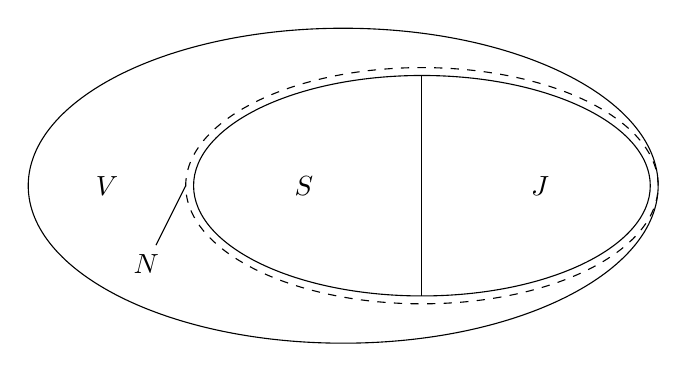
\begin{tikzpicture}
    \draw (0,0) circle [x radius = 4cm, y radius = 2cm];
    \draw (1,0) circle [x radius = 2.9cm, y radius = 1.4cm];
    \draw[dashed] (1,0) circle [x radius = 3cm, y radius = 1.5cm];
    \draw (1,1.4) -- (1,-1.4);
    \node at (-3, 0) {$\m{V}$};
    \node at (-.5, 0) {$\m{S}$};
    \node at (2.5, 0) {$\m{J}$};
    \node at (-2.5, -1) (nnode) {$\m{N}$};
    \draw (-2, 0) -- (nnode) ;
  \end{tikzpicture}
  \caption{Sets}\label{fig:sets}
\end{figure}

To be able to bloom each node separately, we cannot store the boundary edges of a cluster in a single list $\m{L}$ at the cluster. Instead, we store the boundary list for each node $n_i$ separately in their own boundary lists $n_i.\m{L}$. Here we use the $object.property$ notation to indicate that the property is stored at the parent object. As we will see in the next section, the calculation of node-delays is dependant on the direction in which $\m{N}_\alpha$ is traversed. We store the node set by its root $n_r$ at $C_\alpha$. 

\begin{theorem}
  The set of nodes $\m{N} = \{n_1, n_2, .... n_{\nset}\}$ of cluster $C$ is a connected acyclic graph with root $n_r$, and exists next to the exists set of vertices $\m{V}_\alpha$. The function of $\m{N}_\alpha$ is to store the list of boundary edges at the nodes and growing each node according to the calculated node delay.
\end{theorem}


\subsection{Node parity and delay}\label{sec:nodedelay}

The calculation of the PMW for each node in a cluster is a heavy task, as for each node the entire clusters needs to be checked on which edges are part of the matching and results to a quadratic complexity. Luckily, the complexity can be reduced to linear by the calculation of the relative \emph{delay} of each node, where the tree of the node set is traversed.

\subsubsection{1D node tree}

To show how this calculation is performed, we first take the example of a 1D node tree $\nset_{1D}$ of size $S_\nset$, where all nodes lie on one line, but are allowed to grow in x and y directions. In our example, we only look at the first 3 nodes $n_1, n_2$, connected by edge $\epsilon_{1}$, and $n_3$, connected to $n_2$ by edge $\epsilon_{2}$. The node tree continues after $n_3$ for $S_\nset - 3$ nodes. Note that edges of the node set are indicated by $\epsilon$, whereas edges of the vertex set are indicated by $e$. 

Recall that the size of the node $n.s$ is equal to the iterations it has grown, one half-edge per iteration. This means that if a merge with some other cluster occurs on a boundary edge of $n$, the weight of the matchings edges within the flower of $n$ is equal to $\floor{n.s/2}+1$ or. For a merge on $n_1$, we also add edge $\epsilon_2$ and some value $k$ corresponding to the weight of matchings in the remainder of the cluster. Let us calculate the PMW values for each of nodes $n_1, n_2, n_3$.
\begin{eqnarray*}
% \nonumber % Remove numbering (before each equation)
  PMW(n_1) &=& \floor{n_1.s/2}+1 + \epsilon_2 + k \\
  PMW(n_2) &=& \floor{n_2.s/2}+1 + \epsilon_1 + \epsilon_2 + k \\
  PMW(n_3) &=& \floor{n_3.s/2}+1 + \epsilon_1 +k
\end{eqnarray*}
By taking the summed difference in PMW values in subsequent nodes, the relative delay of a node $n.d$ can be calculated with respect to the first node. In this differential, we set $n_1.d$ of the first node to zero.
\begin{eqnarray*}
% \nonumber % Remove numbering (before each equation)
  n_1.d &=& 0 \\
  n_2.d &=& PMW(n_2) - PMW(n_1) + n_1.d = 2(\floor{n_2.s/2} - \floor{n_1.s/2} + \epsilon_1) + n_1.d \\
  n_3.d &=& PMW(n_3) - PMW(n_2) + n_2.d = 2(\floor{n_3.s/2} - \floor{n_2.s/2} - \epsilon_2) + n_2.d
\end{eqnarray*}
These delay values are not entirely correct, as $n_1.s = n_2.s = 2i$ yields the same value as  $n_1.s = 2_i,  n_2.s = 2)i + 1$. We introduce growth support of a node $n.g = n.s \bmod 2$ to accommodate for this degeneracy in PMW, and add this to the delay values.
\begin{eqnarray*}
% \nonumber % Remove numbering (before each equation)
  n_1.d &=& 0 \\
  n_2.d &=& 2\big(\floor{(n_2.s+n_2.g)/2} - \floor{(n_1.s+n_2.g)/2} + \epsilon_1\big) - (n_1.g + n_2.g)\bmod 2 + n_1.d \\
  n_3.d &=& 2\big(\floor{(n_3.s+n_3.g)/2} - \floor{(n_2.s+n_3.g)/2} - \epsilon_2\big) - (n_3.g + n_2.g)\bmod 2 + n_2.d
\end{eqnarray*}
If we were to consider some nodes $n_4, n_5...$ as well, we would find a trend in which the delay calculation is dependant on the \emph{parity} of the node number $i$. The delay of odd node $n_{2i+1}$ has the positive addition of $\epsilon_{2i+1}$ in its delay value, and the substraction of $\epsilon_{2i}$ for an even node $n_{2i}$. Thus we can generalize the delay calculation as the following:
\begin{multline}\label{eq:1ddelay}
n_i.d = n_{i-1}.d + 2\bigg(\floor{\frac{(n_i.s+n_i.g)}{2}} - \floor{\frac{(n_{i-1}.s+n_i.g)}{2}} + (-1)^{i+1}\epsilon_{i-1}\bigg) \\
         - (n_{i}.g + n_{i-1}.g)\bmod 2 \hspace{.5cm} | \hspace{.5cm} n_0.d = 0.
\end{multline}

Using equation \ref{eq:1ddelay}, we can calculate all the relative delays in the 1D tree by traversing the node tree just once from left to right. The initial delay $n_0.d$ can be set at any arbitrary value, as there may be some odd node $n_i$ in the tree that has $n_i.d < n_0.d$. For each node set, we therefore need to store the \emph{minimal delay value}. This value can be stored at the cluster object $C.d$. To grow a cluster, we first calculate its node delays. Then, in each round of growth, we traverse the node tree to find nodes where $n.w = n.d - C.d$, where $n.w$ is the number of growth iterations a node has \emph{waited}. For all nodes that do not satisfy, we add 1 to its waited value.

\subsubsection{Node tree parity}

The 1D node tree does not accurately represent node trees that occur on a real lattice. On a 2D (Pauli errors) and 3D lattice (Pauli and measurement errors), the node tree is allowed to form in the same dimensions. But as $\nset$ is an acyclic graph, the 3D variant can be considered equal to the 2D variant. The difference is that now the \emph{ancestry} in the tree, the set of parent-child relations, is not determined by some number $i$, and each node can have more than 2 connections.

The delay calculation is done comparatively with the previous node, which means that there must be some directed path within $\nset$, such that there is a clear direction to traverse the tree for the delay calculation. We can start the calculation from the root $n_r$. The node parity, previously determined by the number $i$, is now set by the number of children nodes modulo 2. To calculate this parity for each node without traversing all children nodes, we can use the following function
\begin{equation}\label{eq:nodeparitypart}
  n_\beta.p =
  \begin{cases}
    0, & \mbox{if $n_\beta$ has no children}  \\
    \big( \sum_{j} 1-n_{\gamma,j}.p \big ) \bmod 2 \hspace{.2cm} | \hspace{.2cm} \forall n_\gamma \mbox{ child of } n_\beta, & \mbox{otherwise},
  \end{cases}
\end{equation}
where $n_\beta$ is the node of interest, and each of the nodes $n_{\gamma,j}$ is a child of $n_\beta$. As this requires the parity of each child node to be known, the node parities of the entire set can be calculated by a depth-first search (DFS) of the node tree, and traversing back to the root recursively and applying the above equation.

Since $\nset$ is acyclic, any node in the set can be set as the root $n_r$ of the set, and the calculation of the parity would still be valid, although not identical. The node set $\nset$ is therefore a $semi$-directed tree, in which the edges are undirected, but an ancestry is set by the root node $n_r$. If the root node changes to $n_{r}'$, the ancestry within the tree changes, and the node parities within the set become unknown, or \emph{undefined}, requiring a new calculation of a reversed DFS from $n_{r}'$.

\begin{lemma}\label{lem:anynoderoot}
  Any node $n_i \in \m{N}_\alpha$ is a valid root.
\end{lemma}

\begin{lemma}\label{lem:nodeCalcParity}
  The node parity $n_i.p$ is defined as of the number of children nodes of node $n_i$ modulo 2, and can be calculated via a reversed DFS from root $n_r$. If a new node is set as root $n_r'$, the ancestry in a set changes, rendering node parities within the set to "undefined".
\end{lemma}

\subsubsection{Node tree delay}

The delay equation \ref{eq:1ddelay} can be altered by replacing the node number $i$ with some parent-child relationship between nodes, similarly to the parity calculation. To calculate the node delays within $\nset$, we need to traverse $\nset$ in a second DFS from root $n_r$ with
\begin{multline}\label{eq:2ddelay}
  n_\beta.d = n_\alpha.d + 2\bigg(\floor{\frac{(n_\beta.s+n_\beta.g)}{2}} - \floor{\frac{(n_\alpha.s+n_\beta.g)}{2}} + (-1)^{n_\beta.p-1+1}\epsilon_\beta\bigg) \\
         - (n_\beta.g + n_\alpha.g)\bmod 2 \hspace{.5cm} | \hspace{.5cm} n_r.d = 0, \hspace{.2cm} n_\beta \mbox{ child of } n_\alpha,
\end{multline}
where $n_\beta$ is the node of interest and $n_\alpha$ is an ancestor of $n_\beta$, and the sign of the edge component is now dependant on the node parity $n.p$. As the node parities are only defined while the same node is root per lemma \ref{lem:nodeCalcParity}, the delay calculation is only valid if the DFS is performed from the same root $n_r$ as in the parity calculation.

\begin{lemma}\label{lem:nodecalc_ancestrypath}
 The calculation of node delays is only valid while node parities within the set are defined along the same ancestry as the node delay calculation.
\end{lemma}

An interesting aspect of the node delays is that the relative differences in delays in neighboring nodes are the some for any node as root $n_r = n \forall n \in \nset$. The actual delay value may differ for different roots as we always set $n_r.d =0$. This is the reason that when blooming a node, we check for $n.w = n.d - C.d$, as $n.d - C.d$ for each node is the same for any node as root. This fact strengthens lemma \ref{lem:anynoderoot}. 

\subsubsection{Junction node parity and delay}

Up until now, we have neglected junction-nodes in our story on node parity and delays. But as junction nodes have the same properties as syndrome nodes, there also exists edges seeded in junction nodes, and thus they must be included in the parity and delay calculations. Furthermore, without junction nodes, lemma \ref{lem:anynoderoot} cannot be true for a node set $\nset$ for all nodes $n \in \nset$ for the same set of edges $\{\epsilon\}$.

As a junction node is also allowed to bloom, similarly to a syndrome node, equation \ref{eq:2ddelay} still holds for junction nodes. However, the parity of a junction node is calculated differently. Consider an example node set $\nset_e$ with 5 syndrome nodes $\{\sigma_1,...,\sigma_5\}$ lined up linearly with distance 1 between them and $n_r = \sigma_1$. Let us drop the $n.s, n.g$ components of the delay in equation \ref{eq:2ddelay} as we are now only interested in the parity component $(-1)^{n_\beta.p-1+1}\epsilon_\beta$. The parity of $\sigma_4$ is odd, therefore
\begin{equation*}
  \sigma_4.d = \sigma_3.d + 2(\sigma_3, \sigma_4),
\end{equation*}
where $\epsilon = (\sigma_3, \sigma_4)$ is an edge connecting two nodes.

Consider now a second example node set $\nset_e'$ with 3 syndrome nodes and 2 junction nodes $\{\sigma_1, j_2, \sigma_3, j_4, \sigma_5\}$. The PMW's for $\sigma_3$ and $j_4$ are $(\sigma_1, j_2) + (j_4, \sigma_5)$ and  $(\sigma_1, j_2) + (\sigma_3, j_4) + (j_4, \sigma_5)$, respectively, where the delay in $j_4$ is now
\begin{equation*}
  j_4.d = \sigma_3.d - 2(\sigma_3, j_4).
\end{equation*}

We see that the edge component of the delay calculation now has an opposite sign. This flip in sign is due to a flip in node parity for junction nodes compared to syndrome nodes. As a result, we can generalize the parity calculation of equation \ref{eq:nodeparitypart} for realistic node sets.
\begin{equation}\label{eq:nodeparity}
  n_\beta.p =
  \begin{cases}
    0, & \mbox{if $n_\beta$ has no children}  \\
    \big( \sum_{j} 1-n_{\gamma,j}.p \big ) \bmod 2 \hspace{.2cm} | \hspace{.2cm} \forall n_\gamma \mbox{ child of } n_\beta, & n_\beta \equiv \sigma_\beta \\
    1 - \big( \sum_{j} 1-n_{\gamma,j}.p \big ) \bmod 2 \hspace{.2cm} | \hspace{.2cm} \forall n_\gamma \mbox{ child of } n_\beta, & n_\beta \equiv j_\beta
  \end{cases}
\end{equation}

To put this into perspective of lemma \ref{lem:nodeCalcParity}, the parity of a syndrome node is the number of children \emph{syndrome} nodes. The parity of a junction node is 1 minus the number of children syndrome nodes. From here, our definition of parity and delay calculation stays unchanged; the parities can to be calculated by a reversed DFS of the node tree from the root with equation \ref{eq:nodeparity}, and the delays by a second DFS with equation \ref{eq:2ddelay}.

\begin{lemma}\label{lem:nodecalc_junction}
  The node parity in a syndrome node $\sigma.p$ is the number of children syndrome nodes $\sigma_\gamma$ modulo 2. The node parity in junction node $j.p$ is 1 minus the above definition.
\end{lemma}

To perform a reverse DFS of the node tree, we can use a \emph{head recursive} function that calls itself, where the recursiveness is before the required routine. The parity calculation is then the following algorithm.
\begin{algo}[algotitle=CalcParity, label=al:calcparity]
\begin{algorithm}[H]
\SetKwData{node}{node}
\SetKwData{cluster}{cluster}
\SetKwData{child}{child}
\SetKwData{parity}{parity}
\SetKwData{pary}{p}
\SetKwFunction{cp}{CalcParity}
\SetKwFunction{summation}{Sum}

\KwData{\node}
\KwResult{Defined parities for all children of \node}

\BlankLine

\parity $=$ \summation{$[1 - $ \cp{\child} $\forall$ \child of \node $]$} $\%2$\;
\uIf{\node $\equiv \sigma$}{
    \node.\pary $=$ \parity}
\uElseIf{\node $\equiv j$}{
    \node.\pary $= 1-$ \parity}
\KwRet{\node.\pary}
\end{algorithm}
\end{algo}


\subsubsection{Degree of delay due to parity inversion }

With equation \ref{eq:2ddelay}, we can calculate the appropriate delays in nodes such that if the bloom in these nodes are delayed for that many iterations, the PMW's for every node in the set is equal. We will see how to grow a node set in section \ref{sec:growingcluster}. After that, we will see how to join two node sets in the case of a merge of two clusters in section \ref{sec:jointnodesets}. But before we move on, we already see a problem arising in the parity and delay calculations.

If some odd number of nodes $\nset_o$ is attached to $n^e$ of $\nset_e$ during a join operation of two node sets, node parities for nodes in subset $\nset_e'= \{n_i \in \nset_e | n_i \mbox{ ancestor of } n^e\}$ are flipped, where odd nodes become even and even become odd, which is called \emph{parity inversion}. Per lemma \ref{lem:nodecalc_ancestrypath}, the delays in $\nset_e'$ are now undefined and need to be recalculated. If before the join operation, $\nset_e$ had grown for some iterations where the odd nodes have waited (approaching equal PMW), the even nodes will have some node sizes larger than the odd node sizes $n^e_{even}.s > n^e_{odd}.s$. After the join operations, the parities for nodes in $\nset_e'$ flip, and now the previously-even odd nodes have some positive delay. As $n^e_{even}.s > n^e_{odd}.s$, these delays will increase in value per equation \ref{eq:2ddelay} compared to the previous delay calculation.

As the lattice increases in size, the number of merges between clusters or join operations between node sets will also increase. The node parities for some parts of some node sets will suffer parity inversion during these merges, leading to increasingly larger delay values. The delayed bloom of nodes may therefore not be balanced at all with the current delay equation. We therefore introduce a parameter $K_{bloom} \in [0, 1]$ that determines the degree of delay of a node.

\begin{multline}\label{eq:delayequation}
  n_\beta.d = n_\alpha.d + \Bigg \lceil K_{bloom} \Bigg( 2\bigg(\floor{\frac{(n_\beta.s+n_\beta.g)}{2}} - \floor{\frac{(n_\alpha.s+n_\beta.g)}{2}} + (-1)^{n_\beta.p-1+1}\epsilon_\beta\bigg) \\
   - (n_\beta.g + n_\alpha.g)\bmod 2 \Bigg) \Bigg \rceil \hspace{.3cm} | \hspace{.3cm} n_r.d = 0, \hspace{.2cm} n_\beta \mbox{ child of } n_\alpha,
\end{multline}

From intuition the degree of delay should be set to $K_{bloom} = 1/2$. For this value, the delays in a node set are halved, such that in the case of parity inversion, the delay values from before and after the inversion are kept at minimum. But as the inversion of parities mostly does not occur on all nodes in a set, this is not necessarily true, and other values of $K_{bloom}$ should be explored.

\begin{lemma}
  The degree of delay $K_{bloom}$ determines the part of the calculated delays that is actually assigned to the nodes. This is to minimize the node delays in new delay calculations in nodes that have suffered parity inversion after a join operation with another node set.
\end{lemma}

The delay calculation is done by a DFS of the node tree, which can be done by a \emph{tail recursive} function. Here the recursiveness is after the routine, which satisfies the DFS. The delay calculation is then the following algorithm.

\begin{algo}[algotitle=CalcDelay, label=al:calcdelay]
\begin{algorithm}[H]
\SetKwData{node}{node}
\SetKwData{cluster}{cluster}
\SetKwData{child}{child}
\SetKwData{delay}{d}
\SetKwFunction{cdelay}{CalcDelay}

\KwData{\node, \cluster}
\KwResult{Defined parities for all children of \node}

\BlankLine

\If{\node has an ancestor}{
  calculate \node.\delay with equation \ref{eq:delayequation}\;
  \If{\node.\delay $<$ \cluster.\delay}{
    \cluster.\delay $=$ \node.\delay
    }
  }
\For{\child of \node}{
  \cdelay{\child, \cluster}
}
\end{algorithm}
\end{algo}


\subsubsection{Parity and delay routines}

With equation \ref{eq:nodeparity} and \ref{eq:delayequation}, we now finally have the tools to formulate the algorithms to calculate the node parities and delays. For a node set with root $n_r$, we can calculate the parities by calling the head recursive function \codefunc{CalcParity} on $n_r$ in algorithm \ref{al:calcparity}, where we do a reverse DFS of the node tree. The node delays are calculated by calling the tail recursive function \codefunc{CalcDelay} in algorithm \ref{al:calcdelay}, where we do a second DFS of the node tree.

\begin{theorem}
  To prepare a cluster with node set $\m{N}$ and node root $n_r$ with undefined node parities and delays, we calculate node parities in $\m{N}$ by calling the head recursive function $\codefunc{CalcParity}(n_r)$, and sequentially calculate node delays in $\m{N}$ by calling the tail recursive function $\codefunc{CalcDelay}(n_r)$.
\end{theorem}


\subsection{Growing a cluster}\label{sec:growingcluster}

The boundary list for each cluster is not stored at $C$, but separately stored at each of the nodes $n_i$ in $\m{N}$. To grow a cluster $\codefunc{Grow}(C)$, we now traverse all $n_i \in \m{N}$ from the root $n_r$ and apply $\codefunc{Bloom}(n_i)$, which increases the support of all boundary edges in $\m{L}_{n_i}$ at node $n_i$ by 1. If this node hasn't waited enough $n_i.w - n_i.d - C.d > 0$, we skip this node, add to the wait $n_i.w = n_i.w +1$ and apply \codefunc{Bloom} on its children. New vertices $v_{new}$ grown from node $n_i$ are added to $\m{V}$, while storing the seed node at each new vertex $v_{new}.n = n_i$. New boundary edges are appended to the boundary list $n_i.\m{L}$ stored each seed node $n_i$. The number of nodes in $\m{N}$ and the shape of the flower bush tree therefore does not change while no merge between clusters has happened.

\begin{theorem}\label{the:grownode}
  A cluster $C$ is grown by calling $\codefunc{Bloom}(n_r)$, which first checks for the wait of the current node $n_i.w - n_i.d - C.d> 0$ to grow its boundary edges, and then recursively applies \codefunc{Bloom} to its children.
\end{theorem}

\subsection{Joint of node sets}\label{sec:jointnodesets}
With the addition of the node set $\m{N}$, during a union of clusters $C_\alpha$ and $C_\beta$, we have to additionally combine the node sets $\m{N}_{\alpha}$ and $\m{N}_\beta$. Let us first make a clear distinction between the various routines. On the vertex set $\m{V}$ we apply $\codefunc{Union}(v^\alpha, v^\beta)$, on the two vertices spanning the edge connecting two clusters. On node set $\m{N}$, we introduce here $\codefunc{Joint}(n^\alpha, n^\beta)$, which is called on the two nodes $n^\alpha, n^\beta$ that seeds vertices $v^\alpha, v^\beta$, respectively. From now on, when we talk about the "merge clusters $C^\alpha$ and $C^\beta$", "the union of vertex sets $\m{V}_\alpha$ and $\m{V}_\beta$" or the "joint of node sets $\m{N}_{\alpha}$ and $\m{N}_\beta$", we always refer to the combination of these two routines.

Within the vertex set $\m{V}$, we apply \emph{path compression} and \emph{weighted union} to minimize the depth of the tree and therefore minimizing the calls to the \codefunc{Find} function. Similarly, in the node set $\m{N}$, we would also like to apply a set of rules to minimize the calls to \codefunc{CalcParity} and \codefunc{CalcDelay}. As the structure of the tree is crucial in computing the parities and relative delays between the nodes, these rules will be quite different than in vertex set $\m{V}$. First of all, we note that while the node set does not change, the parities and delays within the node set stay valid.


\begin{lemma}\label{lem:nodesetunchanged}
  While node set $\nset$ is unchanged, the calculated parities and delays within the set are valid.
\end{lemma}

Our rules will be dependant on the parities of the joining node sets, which is the number of syndrome-nodes in the set modulo 2. This is due to that junction-nodes do not add to the count of the number of children nodes per lemma \ref{lem:nodecalc_junction}. Note that the parity of a node set $\m{N}.p$ is therefore exactly the same as the parity of a cluster $C.p$, which also refer to the number of syndromes in the cluster.

\begin{lemma}
  The parity of node set $\m{N}.p$ is the number of syndrome-nodes $a_i \in \m{N}$ modulo 2. The parity of node set $\m{N}.p$ is analogous to cluster parity $C.p$.
\end{lemma}

\subsubsection{Joint to even node set}

Let us first consider the joint operation of two or more node sets, where the resulting node set $\m{N}_{e}$ is even. If we calculate the parities of a node set with even parity $\m{N}_e$, we will end up with an odd node $n_r.p=0$ as root of node set $\m{N}_e$. It therefore does not make sense to talk about node parities within an even node set. Luckily, but not coincidentally, if a node set is even, the cluster is even and therefore will not grow. We could say that we need not to worry about the parties and delays within $\m{N}_{e}$.

\begin{lemma}\label{lem:nodecalc_even}
  Node parities become undefined if multiple node sets joins into a new set $\m{N}$ with even parity.
\end{lemma}

However, it is entirely possible that another cluster grows, and merges onto the cluster of $\m{N}_{e}$. In that case, we might think about recovering some of the node parities and delays that were calculated in the subsets of $\m{N}_e$, such that we don't have to traverse $\m{N}_{e}$ entirely for its parities and delays.

\subsubsection{Joint to odd node set}

Consider the joint operation of an even $\m{N}^e$ and an odd node set $\m{N}^o$ in nodes $n^e, n^o$ respectively, and assume that this joining is due to the growth of odd cluster $\m{N}^o$ onto an "idle" $\m{N}^e$. The joint of these two sets leaves a new odd node set $\m{N}_{new}^o$ with subsets $'\nset^e$ and $'\nset^o$, referring to the original node sets. We are provided with two choices, a) make $n^e$ child of $n^o$, or b) make $n^o$ child of $n^e$. Note that the child node $n^c$ will become the \emph{sub-root} in subset $'\m{N}^c$, where the ancestry in the subset has been reset in the new sub-root, and is allowed per lemma \ref{lem:anynoderoot}.

If the subset $'\m{N}^e$ consists of only two odd node sub-subsets $''\m{N}^o_0, ''\m{N}^o_1$, where $n_0, n_1$ are the joining nodes, the ancestry in $''\m{N}^o_0$ is preserved and $n_1$ is the sub-root of $''\m{N}^o_1$. We see that the parities in all ancestors of $n_0$ are flipped. Let's consider the cases and find whether we can minimize the parity and delay calculation in $'\m{N}^{e}$.

For case a), an even number of nodes of $'\m{N}^e$ is attached to $n^o$, and the ancestry in $'\m{N}^o$ hasn't changed. This means that the parities in $'\m{N}^o$ do not change per lemma \ref{lem:nodeCalcParity}, and the delays in $'\m{N}^o$ are still valid as per lemma \ref{lem:nodecalc_ancestrypath}. In $'\m{N}^e$, as the ancestry path has changed, we are certain to traverse $'\m{N}^e$ from the sub-root $n^e$ to calculate the delays in this subset which is in the order of $S_{'\m{N}^e}$.

In case b), as an odd number of nodes of $'\m{N}^o$ is attached to $n^e$, it means that parities of all ancestor of $n^e$ are flipped. As the ancestry in $'\m{N}^{o}$ has changed, we are certain to traverse $'\m{N}^o$ from the sub-root $n^o$ to calculate the delays which is in the order of $S_{'\m{N}^o}$. The node parity changes in $'\m{N}^e$ will be dependant on the location of $n^e$ in the ancestry compared to $n^1$ and $n^2$, and all children nodes of these parity changes will have to recalculate their delays. Let's call the number of nodes needs to calculate parity and delays in $'\m{N}^e$ a value $S_e \leq S_{'\m{N}^e}$, leaving the total number of operations in the order of $S_e + S_{'\m{N}^o}$.

For $'\m{N}^e$ consisting of two subsets, keeping track of the parity changes between $n^e$, $n^0$ and $n^1$ is still an easy task, and we might gain in minimization in operations in case b) compared to case a) for some value $S_e$ such that $S_e + S_{'\m{N}^o} < S_{'\m{N}^e}$. But as the number of subsets in $'\m{N}^e$ increases, the task of finding the ancestry paths of parity changes becomes analogous to traversing $'\m{N}^e$ entirely $S_e \rightarrow S_{'\m{N}^e}$. To simplify, we always choose case a.

\begin{theorem}\label{the:nodejoint}
  The union of node sets $\m{N}^\alpha, \m{N}^\beta$ on nodes $n^\alpha, n^\beta$ respectively is performed with $\codefunc{Joint}(n^\alpha, n^\beta)$. If the resulting node set $\m{N}$ is odd, one of $\m{N}^\alpha$ and $ \m{N}^\beta$ is odd while the other is even, and $\codefunc{Joint}(n^\alpha, n^\beta)$ makes the node of the even set $n^e$ a child of the node of the odd set $n^o$. If the resulting node set $\m{N}$ is even, the choice is arbitrary.
\end{theorem}



\subsection{Multiple joints per bucket}

Clusters with same vertex set size $S_\vset$ lie in the same bucket $b_i$ and thus are grown together per theorem \ref{the:bucket_order}. Let's call the growth of all clusters in a bucket a \emph{growth iteration}. As the state of fully grown edges are only checked after each growth iteration including possibly many clusters, there may be multiple joint events within the same growth iteration. If the node parities and delays are to be calculated on all the union events in the fusion list $\m{F}$, some node parity and delay calculations may be invalid and unnecessary.

Consider an example with 5 odd clusters $C_1, ... C_5$ with node sets $\nset_1, ... \nset_5$. The union of $C_1$ and $C_2$ to $C_{12}$ is odd-odd and requires no parity-delay calculation. The union of $C_{12}$ and $C_3$ is even-odd, and we calculate the parities and delays in the $\nset_{12}$. The union of $C_{123}$ and $C_4$ is odd-odd and the union of $C_{1234}$ and $C_5$ is even odd, and we calculate the parities and delays in $\nset_{1234}$. The earlier computation in $\nset_{12}$ was therefore unnecessary and possible invalid.

To circumvent this even parity multiplicity, we must make sure to only apply the calculation to the largest even node set in some sequence of joint operations. To do this, we first note that some odd node set $\nset^o$ must always consist of some odd part $'\nset^o$ and an even part $'\nset^e$. The even part $'\nset^e$ may be subdivided into a number of odd and even sub-subsets, as long as the sum is even.
\begin{lemma}\label{lem:oddisevenodd}
  An odd node set $\nset$ that is the result of some joint operations must consist of an odd subset $'\nset^o$ and an even subset $'\nset^e$, where the even subset $'\nset^e$ may consist of smaller sub-subsets $''\nset$.
\end{lemma}
This even subset $'\nset^e$ is the undefined part of $\nset^o$ in which we must calculate the parities and delays. As we can only be sure that the subset $'\nset^e$ is complete after all unions of clusters are complete, we cannot apply and parity-delay calculations during the unions. We suspend these calculations as much as possible by doing them just before a cluster is grown from a bucket.

\begin{lemma}\label{lem:delaywhengrown}
  Parity and delay calculations are only performed on a the undefined part of a node set when a cluster is grown, not directly after a joint operation.
\end{lemma}

The only task now is to store where the even subset $'\nset^e$ starts in the ancestry of subset $\nset^o$.  For each joint operation between odd node set $'\m{N}^o$ and even node set $'\m{N}^e$ on nodes $n^o, n^e$ per theorem \ref{the:nodejoint}, we store the sub-root $'n^e_r$ of subset $'\m{N}^e$ to a list $\m{C}$ at the root node of the resulting set $\m{N}^{res}$ of cluster $C^{res}$. If cluster $C$ is selected for growth as per theorem \ref{the:bucket_order}, we first check for nodes in ${n^r}.\m{C}$ at root and apply $\codefunc{CalcParity}(n_i)$ and $\codefunc{CalcDelay}(n_i)$ for all nodes $n^i \in {n^r}.\m{C}$ to calculate parities and delays in undefined parts of the set. We then call $\codefunc{Bloom}(n_r)$ per theorem \ref{the:grownode}.

\begin{theorem}\label{the:delayonce}
  Undefined parts of an odd node set $\nset^o$ are defined as a set $\m{C}_{\nset^o}$ of sub-roots from which all children (including sub-roots) are undefined, and is stored at root node $n^o_r$. If before it has grown, node set $\nset^o$ is joint with another odd node set, which then act as the even set $\pre{\uparrow}\nset^e$ in a larger joint event, the sub-root of $\pre{\uparrow}\nset^e$ is stored at $n^{\pre{\uparrow}\nset^o}_r$. Delay and parity calculations will then traverse all undefined paths only once.
\end{theorem}

\subsection{Pseudocode}

\subsection{Complexity of Balanced Bloom}

The contribution to the time complexity of the UF-EG decoder compared to the UF-decoder can be divided into two parts. First is the contribution by \codefunc{CalcParity} and \codefunc{CalcDelay}. As these two functions are always called together per theorem \ref{the:delayonce}, we can just introspect the number of calls to one of them, and call this contribution the \emph{delay} complexity. The second contribution will be caused by \codefunc{Grow}, as now we have to additionally traverse the node set tree's of each cluster to access its boundary edges and grow them with \codefunc{Bloom} as compared to a single boundary list per cluster. We call this second contribution the \emph{bloom} complexity.

\subsubsection{Delay complexity}

Consider an odd cluster represented by node set $\pre{k-1}\nset^o$ with set size $S_{\pre{k-1}\m{N}^o}$ that is the result of union between a number of clusters $\pre{k}C_i$ with node subsets $\pre{k}\nset_i$. Here $k$ indicates a \emph{generation}, where larger $k$ indicates a more distant descendent generation of smaller clusters. As $\pre{k-1}\nset^o$ is odd, it will be selected for growth. And because it consists of a number of subsets, $\pre{k01}\nset^o$ is bound to consist of an odd subset $\pre{k}\nset^o_0$ and an even subset $\pre{k}\nset^e$ (lemma \ref{lem:oddisevenodd}) on which we are to calculate the parities and delays (theorem \ref{the:delayonce}).

\paragraph{Fragmentation of a node set}

Let us call this division of odd set into smaller odd and even subsets the \emph{partial fragmentation} $f_1$ of $\pre{k-1}\nset^o$. We can apply another partial fragmentation $f_2$ of $\pre{k}\nset^e$ into 2 odd subsets $\m{F}'_k=\{\pre{k}\nset^{o}_1, \pre{k}\nset^{o}_2\}$, and call the 2 fragmentations $f_1, f_2$ of $\pre{k}\nset^o$ into a set of node sets $\m{F}_k = \{\pre{1}\nset^o_0, \pre{1}\nset^{o}_1, \pre{1}\nset^{o}_2\}$ a \emph{fragmentation step} $f$. Each odd subset $\pre{k}\nset^o_i$ of $\m{F}_k$ can continue to be partially fragmented by $f_1$ into $\pre{k+1}\nset^{o,o}_{i, 0}$ and $\pre{k+1}\nset^{o,e}_i$ the same way. Note that a node set $\nset^o$ can only be fragmented if $S_{\nset^o} \geq 3$, in which case the resulting subsets have size 1.

\begin{lemma}\label{lem:partialfrag}
  Let the separation of an odd node set $\pre{k-1}\nset^o$ into subsets $\m{F}_k'=\{\pre{k}\nset^o_0, \pre{k}\nset^e\}$ be the partial fragmentation $f_1$ and subsequently into subsets $\m{F}_k= \{\pre{k}\nset^o_0, \pre{k}\nset^{o}_1, \pre{k}\nset^{o}_2\}$ be $f_2$ of $\nset$. The combination of the two is a fragmentation step $f$.
  \begin{equation}\label{eq:partialfrag}
    \m{F}_k = f(\pre{k-1}\nset^o) = f_2(f_1(\pre{k-1}\nset^o)) = f_2(\{\pre{k}\nset^o_0, \pre{k}\nset^e\}) = \{\pre{k}\nset^o_0, \pre{k}\nset^{o}_1, \pre{k}\nset^{o}_2\} \hspace{.3cm} | \hspace{.3cm} S_{\pre{k}\nset^o_i} \geq 3
  \end{equation}
\end{lemma}

Each odd node set of $\m{F}_k$ can undergo the same fragmentation step into odd subsets, leaving us again with a set of node subsets $\m{F}_{k+1}$. We can do this some $p$ times until our resulting set of node sets $\m{F}_{p}$ consists only of smallest possible node subsets $\nset^o$ where $S_{\nset^o}=1$. To find the worst case complexity, we want to maximize the delay complexity within $\pre{k-1}\nset^o$; we are to find the sequence of joint operations that maximizes the sum of even node sets sizes $S_{\nset^e}$ in all partial fragmentations in the \emph{full fragmentation} $F$ of $\nset^o$.

Looking at the fragmentation from the other way, we have a set of size 1 node sets that undergo joint operations in each partial fragmentation. In $f_2$, two odd node sets join, and we do not add to the count of $N_delay$. In $f_1$, an odd and an even note sets join, and we have to calculate the delays in the even node set before moving on to the next joint operation.

\begin{lemma}
  Let the full fragmentation of $\nset$ be
  \begin{equation}\label{eq:fullfrag}
    F(\nset^o) = \underbrace{f(f(...f(\nset)))}_\text{p times} = \{\pre{p}\nset^{o}_1, \pre{p}\nset^{o}_1, \pre{p}\nset^{o}_2, ... ,\pre{p}\nset^{o}_{N_\sigma} \} \hspace{.3cm} | \hspace{.3cm} S_{\pre{p}\nset^{o}_i} = 1,
  \end{equation}
  where along each fragmentation step $k$ a partial fragmentation set $\m{F}'_k$ is produced, the number of delay calculations is
  \begin{equation}\label{eq:maxdelay}
    N_{delay} = \sum_{k=1}^{p} \sum \{ S_{\pre{k}\nset^e} | \forall \mbox{ even } \pre{k}\nset^e \in \m{F}'_k \}.
  \end{equation}
\end{lemma}

\paragraph{Partial fragmentation number}
Note that here we ignore the fact that the partial fragmentations of some node set may not result in two but many subsets. Let us call the number of odd subsets the \emph{fragmentation number} $N_f$. For partial fragmentation $f_1$, the separation of the odd node set $\pre{k-1}\nset^o$ must be in 1 odd and 1 even subset per lemma \ref{lem:oddisevenodd}, thus $N_{f_1} = 2$. For partial fragmentation $f_2$, the separation of even set $\pre{k}\nset^e$ can be in $2n_o$ odd and $n_e$ even subsets. But any even subset will be subjected to the same partial fragmentation $f_2$ in the full fragmentation, reducing the fragmentation number to $N_{f_2} = 2n_o$.

To find $N_{f_2} $, let us consider two cases where $n_o = 1$ or $n_o=2$. If an even node set $\nset^e$ is fragmented with $\pre{k}N_{f_2}=2$, a fragmentation step of $f_2, f_1$ will be
\begin{eqnarray*}
% \nonumber % Remove numbering (before each equation)
  \m{F}^e_k &=& \{ \pre{k} \nset^{o}_1, \pre{k} \nset^{o}_2\},  \\
  \m{F}'^e_{k+1} &=& \{\pre{k+1}\nset^{o,o}_{1,0}, \pre{k+1}\nset^{o,e}_1, \pre{k+1}\nset^{o,o}_{2,0}, \pre{k+1}\nset^{o,e}_2 \}.
\end{eqnarray*}
For $N_{f_2} = 4$, a fragmentation step will be
\begin{eqnarray*}
% \nonumber % Remove numbering (before each equation)
  \m{F}^e_k &=& \{ \pre{k}\nset^{o}_1, \pre{k}\nset^{o}_2\,  \pre{k}\nset^{o}_3\, \pre{k}\nset^{o}_4\},  \\
  \m{F}'^e_{k+1} &=& \{\pre{k+1}\nset^{o,o}_{1,0}, \pre{k+1}\nset^{o,e}_1,  \pre{k+1}\nset^{o,o}_{2,0}, \pre{k+1}\nset^{o,e}_2,  \pre{k+1}\nset^{o,o}_{3,0}, \pre{k+1}\nset^{o,e}_3, \pre{k+1}\nset^{o,o}_{4,0}, \pre{k+1}\nset^{o,e}_4 \}.
\end{eqnarray*}

If the size of $S_{\nset^e}$ is large enough, and we fragment in the same ratio (see next paragraph), the sum of even node set sizes in these two kinds of fragmentations will be the same. However, the number of subsets in each fragmentation step has increased by a factor of 2, which means that the average size of subsets have decreased by 2. Consequently, the node set size decreases faster towards the minimum size of 3 as more fragmentation steps are applied. As the sum of even node set sizes in each fragmentation step is the same, increasing $N_{f_2}$ will decrease the number of fragmentation steps and thus the number of delay calculations $N_{delay}$ per equation \ref{eq:maxdelay}. Thus our decision of $N_{f_2}=2$ in lemma \ref{lem:partialfrag} is correct.

\paragraph{Partial fragmentation ratio}
To complete the fragmentation description, we will need to find the fragmentation ratios $R_0, R_1, R_2$ of a fragmentation step. The fragmentation ratios determine the node set sizes of the subsets in $\m{F}_{k-1}$ with respect to the size of $\pre{k}\nset^o$, where $R_i S_{\pre{k-1}\nset^o}$ is the size of subset $\pre{k}\nset^o_i$. Note that $R_0$ corresponds to the odd subset from $f_1$, and $R_1, R_2$ to the odd subsets in $f_2$.

\begin{lemma}\label{lem:fragratio}
  Let the fragmentation ratios $R_0, R_2, R_2$ be the relative set sizes of the odd subsets in the fragmentation set $\m{F}_{k} = \{\pre{k}\nset^o_0, \pre{k}\nset^{o}_1, \pre{k}\nset^{o}_2 \}$ with respect to set $\pre{k-1}\nset^o$, where
  \begin{equation}\label{eq:fragratio}
    R_j = \frac{S_{\pre{k}\nset^o_j}}{S_{\pre{k-1}\nset^o}}
  \end{equation}
\end{lemma}

Recall lemma \ref{lem:delaywhengrown} that the delay calculations are only done before a cluster is grown. During this grow process, some $n_v$ vertices are added to the cluster, and some union or joint operations can occur. If no joint operations occur, the node set stays unchanged, and the cluster is allowed to continue growth without delay calculations per lemma \ref{lem:nodesetunchanged}. We want to minimize $n_v$, as each added vertex here is not a node that can possibly count towards $N_{delay}$, and it is therefore preferable that some joint operations do occur during growth.

Take the first fragmentation sets $\m{F}'_{k} = \{\nset^o_0, \nset^{e} \}$ and $\m{F}_{k} = \{\nset^o_0, \nset^{o}_1, \nset^{o}_2 \}$ of some cluster defined by node set $\pre{k-1}\nset^o$. These partial fragmentation correspond to 2 joint operations, between two odd clusters $ \nset^{o}_1, \nset^{o}_2 $ in $f_2$, and between odd and even clusters $\nset^o_0, \nset^{e} $ in $f_1$.

If we want to minimize $n_v$ in $f_2$, these odd clusters must grow within the same bucket $b_i$, which means that $S_{\vset_1} = S_{\vset_2}$. Note that these are the cluster sizes and not node set sizes. For $f_1$, the joint event is caused by growth of $\nset^o_0$ in either some bucket $b_j > b_i$ where $ S_{\vset_0} > S_{\vset_1} $, or growth in the same bucket $b_i$ where $S_{\vset_0} = S_{\vset_1} $. This leaves us with $S_{\vset_0} \geq S_{\vset_1} = S_{\vset_2}$.

To maximize $N_{delay}$, we want to maximize $S_{\nset^e} = S_{\nset^o_1} + S_{\nset^o_2}$ in $f_1$. Recall from equation \ref{eq:sets} that $S_\nset \leq S_\vset$. We assume the largest possible node set size $S_\nset = S_\vset$ to find that $ S_{\nset^e} $ is largest if $S_{\vset_0} = S_{\vset_1}$. We can therefore conclude that $S_{\nset^o_0} = S_{\nset^o_1} = S_{\nset^o_2}$ and $R_0 = R_1 = R_2 = \frac{1}{3}$

\begin{lemma}\label{lem:thirdratio}
  A fragmentation step of $\pre{k-1}\nset^o$ is maximized in $S_{\pre{k}\nset^e}$ if the fragmentation ratios take the values $R_j = \frac{1}{3}$.
\end{lemma}

\paragraph{Time complexity}

To find the time complexity cased by the delay calculations, we are left with a single variable $p$, the number of fragmentation steps that can be taken. If we assume that in each growth step not a single non-node vertex is added $n_v = 0$, the full fragmentation of some node set $\nset^o$ is just the continuous division of the set in 3 parts per lemma \ref{lem:thirdratio}, which can be calculated easily.
\begin{equation}\label{eq:numfrag}
  p = \log_3(S_{\nset^o})
\end{equation}
In each fragmentation step $\m{F}'_k$, $f_1$ is equivalent to the joint of odd node sets with even node sets where the sum of odd sets sizes is
\begin{equation}\label{eq:sumoddsetsize}
  \sum \{ S_{\pre{k}\nset^o} | \forall \mbox{ odd } \pre{k}\nset^o \in \m{F}'_k \} = \frac{1}{3}S_{\nset^o},
\end{equation}
and the sum of even node set of sizes is
\begin{equation}\label{eq:sumevensetsize}
  \sum \{ S_{\pre{k}\nset^e} | \forall \mbox{ even } \pre{k}\nset^e \in \m{F}'_k \} = \frac{2}{3}S_{\nset^o}.
\end{equation}
This approximation is true as we have taken $S_\nset = S_\vset$ and $n_v=0$. Filling in equation \ref{eq:numfrag} and \ref{eq:sumevensetsize} in \ref{eq:maxdelay}, we find that

\begin{eqnarray}
% \nonumber % Remove numbering (before each equation)
\nonumber  N_{delay} &\leq& \sum_{k=1}^{p} \sum \{ S_{\pre{k}\nset^e} | \forall \mbox{ even } \pre{k}\nset^e \in \m{F}'_k \}. \\
\nonumber   &=& \sum_{k=1}^{\log_3(S_{\nset^o})} \frac{2}{3}S_{\nset^o} \\
   &=& \frac{2}{3}S_{\nset^o}\log_3(S_{\nset^o})
\end{eqnarray}

The node set size of set $\nset^o$ is bounded by the lattice size $N$. The worst case time complexity of the delay computation is bounded by $\m{O}(N\log_3(N))$. The real worst-case complexity is even lower as it is quite certain that not all vertices are nodes such that $S_\nset < S_\vset$ and $n_v > 0$.

\subsubsection{Bloom complexity}

To grow a cluster represented by a node set $\nset$, we have to traverse the entire set from root to stem to iterate over each boundary list that are stored at the nodes. Let's call the total number of times any node is traversed by \codefunc{Bloom} $N_{bloom}$.

Similar to the previous section we make the assumption of a maximum number of nodes on the lattice where in each cluster $S_\nset = S_\vset$ and $n_v = 0$. Recall that every odd node set $\pre{k}N^o_i$ in each fragmentation set $\m{F}_k$ is subjected to growth in each partial fragmentation, and that we start out with a maximum number of smallest cluster of size $S_{\pre{p}\nset} = S_{\pre{p}\vset} = 1$. Thus we are certain that with this assumption we have the upper bound in $N_{bloom}$.
\begin{equation}\label{eq:nnode}
  N_{bloom} \leq \sum_{p}^{k=1}\sum \{ S_{\pre{k}\nset} | \pre{k}\nset \in \m{F}_k \}
\end{equation}
For a full fragmentation of $\nset$ of size $S_\nset$, the sum of all set sizes in each fragmentation set $\m{F}$ is
\begin{equation}\label{eq:sumsetsfrag}
  \sum \{S_{\pre{k}\nset} | \pre{k}\nset \in \m{F}_k \} = S_\nset.
\end{equation}
By filling in $p$ we find that
\begin{eqnarray}
% \nonumber % Remove numbering (before each equation)
  \nonumber N_{bloom} &\leq& \sum_{p}^{k=1}\sum \{ S_{\pre{k}\nset} | \pre{k}\nset \in \m{F}_k \} \\
  \nonumber &=& \sum_{k=1}^{\log_3(S_{\nset^o})} S_\nset \\
   &=& S_{\nset^o}\log_3(S_{\nset^o}),
\end{eqnarray}
which again corresponds to a worst case time complexity that is bounded by $\m{O}(N\log_3(N))$.

\subsection{Boundaries}

\subsection{Erasure noise} 